\documentclass{amsbook}

\usepackage[
    a5paper,
    margin=28mm,
    marginparwidth=20mm,
    marginparsep=3mm
]{geometry}

\usepackage[
    a5paper,
    margin=28mm,
    marginparwidth=20mm,
    marginparsep=3mm]{geometry}

\usepackage{
    verse,
    microtype,
    mathtools,
    marginnote,
    graphicx,
    ragged2e,
    xstring,
    afterpage,
    pifont
}

\usepackage{fontspec}
\newfontfamily\hoskeroe{English Towne}
\newfontfamily\arabicish[Scale=1.2, Script=Arabic]{KacstQurn}
\newfontfamily\frakturish{Fette UNZ Fraktur}
\setmainfont[
    ItalicFont=cmunti.otf,
    BoldFont=cmunbx.otf,
    BoldItalicFont=cmunbi.otf,
    Numbers=OldStyle
]{cmunrm.otf}

\usepackage{xfrac}
\DeclareInstance{xfrac}{cmunrm.otf(0)}{text}{
    slash-symbol-font = ptm,
    scale-factor=0.8,
    numerator-top-sep = 0pt,
    denominator-bot-sep = 0pt,
    slash-right-kern=-.25em,
    slash-left-kern=-.3em
}

\usepackage[hidelinks]{hyperref}

\hyphenpenalty=1000

% For Arabic text inside left-to-right text.
\newcommand{\textarabic}[1]{\bgroup\textdir TRT\arabicish #1\egroup}

\newcommand{\addpoemtolist}[1]{}
\newcommand{\poeticmarginnote}[1]{\marginnote{\footnotesize #1}}
\newcommand{\poeticfrac}[2]{\sfrac{$#1$}{$#2$}}
\newcommand{\prosesep}{
    \bigskip
    \centerline{\vbox{\hrule width 2in}}
    \bigskip
    \bigskip
}

\newcounter{pageoffset}
\newcounter{pagedifference}
\newcommand\blfootnote[1]{%
    \begingroup
    \renewcommand\thefootnote{}\footnote{#1}%
    \addtocounter{footnote}{-1}%
    \endgroup
}

\newcommand{\poemone}{}
\newcommand{\poemtwo}{}
\newcommand{\poemthree}{}
\newcommand{\printpoems}{%
    \setcounter{pagedifference}{\value{page}-\value{pageoffset}}
    \IfEq{\thepagedifference}{2}
    { \poemone \clearpage}{}
    \IfEq{\thepagedifference}{5}
    {\poemtwo \clearpage
    \poemthree \clearpage}{}
    \afterpage{\printpoems}%
}
\newcommand{\initprintpoems}{
    \setcounter{pageoffset}{\thepage-1}
    \afterpage{\printpoems}
}


\title{The First Book. Lucifer in Starlight}

\begin{document}
\frontmatter
\renewcommand\thefootnote{{}}
\maketitle

\thispagestyle{empty}
\topskip0pt
\vspace*{\fill}
\noindent {\it How you are fallen from heaven, Lucifer, son of the morning. How you are cut down to the ground, you who laid nations low. You said in your heart, I will ascend into heaven; I will exalt my throne above the stars of God; I will ascend above the heights of the clouds; I will make myself like the Most High. But you are brought down to hell, to the depths of the pit...}
\vspace*{\fill}
\clearpage

\tableofcontents

\thispagestyle{empty}
\topskip0pt
\vspace*{\fill}
{\centering
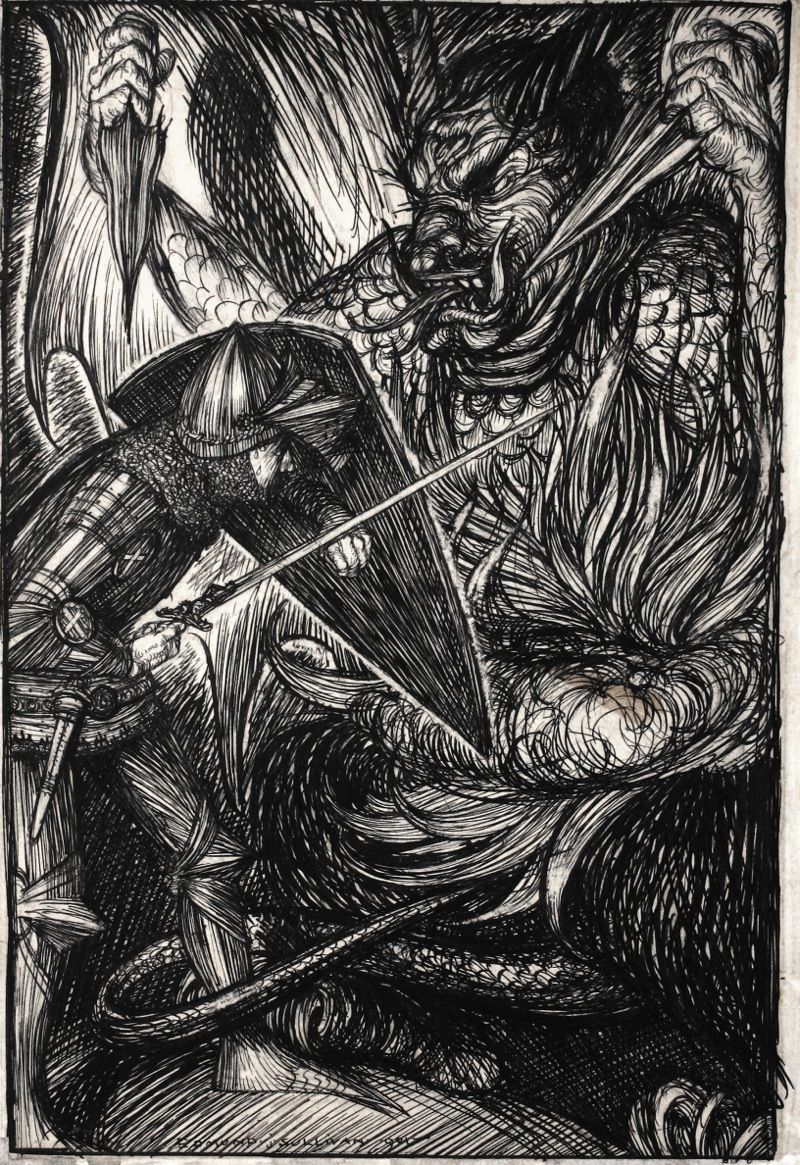
\includegraphics[width=\textwidth]{images/placeholder_image.jpg}}
\vspace*{\fill}
\clearpage

\thispagestyle{empty}
\topskip0pt
\vspace*{\fill}
\noindent {\sc Argument:} {\itshape How the two lovers from \emph{William's Farewell}, having suffered an unrecoverable loss, wandered across the country; and of the strange things that befell them on their way.}
\vspace*{\fill}
\clearpage

\thispagestyle{empty}
\topskip0pt
\vspace*{\fill}
{\centering
\includegraphics[width=\textwidth]{images/autumnal.jpg}}
\vspace*{\fill}
\clearpage

\mainmatter

\chapter{Autumnal}

\renewcommand{\poemone}{
    \begin{figure*}[p!]
\bigskip
\ding{72}
\bigskip
\settowidth{\versewidth}{In the room, we kissed \& drank old fashioneds,}
\begin{verse}[\versewidth]
Afterwards, we drove back to the hotel,\poeticmarginnote{ES}\\*
\vin The lights in the dockyard just coming on\\
And the sun bedding down under the causeway.\poeticmarginnote{Chiswell Beach}\\
\vin The night was heavy with rain and you fell asleep\\*
To something by Snow Patrol or Radio 4.\\!

You blessed the meal when we sat down to supper,\\*
\vin And after, with your hands around the cup.\\
In the room, we kissed \& drank old fashioneds,\\
\vin Watched the first \poeticfrac{1}{2} an hour of {\hoskeroe Heartbreak Ridge};\\*
Then you pulled off your teeshirt with the chinese prints.\\!

I could never admit that I liked it: but\\*
\vin The light from the lampstand gentling your body,\\
A touch of bois des \^iles behind each ear,\\
\vin You laying yourself back on the duvet like\\
You were a teenager and this was the first time.
\end{verse}
\end{figure*}
}
\renewcommand{\poemtwo}{
    \begin{figure*}[p!]
\bigskip
\ding{72}
\bigskip
\settowidth{\versewidth}{In the dark, the heel of my hand found your breastbone,}
\begin{verse}[\versewidth]
I woke up between you \& your sister.\poeticmarginnote{FC}\\*
\vin (When you were kids you'd sleep in the same bunk,\\
So you say; now she's apt to feel jealous.)\\*
\vin All three had fallen asleep in our clothes.\\!

You knelt beside me and gave me my glasses.\\*
\vin Someone stirred and checked through his phone.\\
It was night-time: a rich lampblack dark. In the hallway\\*
\vin Streetlights fondled through the fronds of a birch.\\!

\emph{David} himself would've run out of verses\\*
\vin In praise of that kiss, the deep scar at your waist.\\
In the dark, the heel of my hand found your breastbone,\\*
\vin Guessing its line by touch \& the mind's eye.\\!

Were it not for you I would've missed the snowstorm\\*
\vin Blanching the path down to the weir from the railbridge,\nobreak\\
The emptiness beyond the arbour,\\*
\vin \textsc{Neville}'\textsc{s Cross} and \textsc{Pity Me}.
\end{verse}
\end{figure*}
}
\renewcommand{\poemthree}{
    \bigskip
\centering \ding{58}
\bigskip
\begin{quote}
\poeticmarginnote{Μανασσῆς}God, who in former times heard the petitions of ordinary creatures, take pity on me, and have mercy on the work of your hands. My crimes are so hateful that I have lost the right even to look up and enjoy the sky: the warmth of the sun, and the gentler splendour of the heavens. They weigh me down like a yoke of solid iron, and cling to me like a spiteful shadow. My punishment is more than I can bear; forgive me, Lord. Help me to bend the knee of my heart, and tune my heart strings to your music. Amen.
\end{quote}
}
\initprintpoems
\noindent \textsc{It was}\poeticmarginnote{\frakturish Das Schloß} about four o'clock when we arrived. The fields lay deep in fog. The tarmac of the avenue sped quietly beneath us, marbled with oilslicks and rainwater. It was Edwardian apparently, the house -- all pale stone and subtle volutes. Suzy came out to meet us on the front steps. Her expression was warm, and her hair was a mess.

Then we sat down for tea and cakes. With the big bay window and the grim weather outside, we all felt glad of the fire. I was so nervous, seeing Suzy again after all this time, I lost my appetite, but she wasn't the sort to take offence. Absent friends were toasted. Suzy grilled you excitedly about life back home in Vienna. When we'd finished, you stacked the things up onto the tray, and I carried it out.

In the kitchen, Suzy introduced us to one of the other women, Jess. She must have been half Suzy's age, twice ours -- and yet already there little streaks of grey in her ponytail. She was nice, something of a gentlewoman. She talked in an animated fashion about a faith healing at a recent prayer meeting, emphasising certain points with the knife with which she chopped the onions. I thought how she must have had the lads running after her when she was our age, and wondered if she was married. Then Suzy ushered us into the garden.

Apparently it had been a good year for the jasmine, but it was October now and what hadn't been cut back hung shrivelled and brown. A narrow path ran out across the lawn, down to the river. The cherry tree was full of droplets of rain. Through a plastic window, the shelves of the tool shed presented arms: the tines and blades properly oiled and stacked. I said to myself, It'd be good to find work here, over the spring. Then we came in out of the cold.

A long windowed corridor separated the kitchen from the chapel: a handsome room, oak-panelled and oak-floored, with bean bags spread around the altar. In place of a cross there was a painting of the crucifixion, almost like a photograph. His eyes were bulging, bones visibly broken, the hair on his chest matted with blood. I remembered a passage Suzy had given me on a piece of card during our first acquaintance -- `Christ\poeticmarginnote{Sta Teresa de \'Avila} has no body on earth now but yours' -- then I looked at you. You didn't seem to pay any of it much attention, but perhaps you just kept your eyes lowered out of respect. I find you very hard to read sometimes, and that gets to me.

After that, Suzy took us upstairs to another room. It was as big as the lounge and similarly furnished, but the chairs were laid out in a more formal circle. Suzy said that everyone gathered here every day, first thing in the morning and after supper. In the evenings, the women might want to say sorry for the sins of the day, or tell stories about the things that had happened to them in their lives. There was never any pressure to speak though, she said, nothing to worry about.

There was a library just across the landing: a gorgeous space with a thick red carpet and a stone fireplace. There were eight mahogany bookshelves protruding from the walls, four on the left and four on the right. Then in the centre space, beneath the window, was an enormous copy of \emph{Pilgrim's Progress} laid open on a lectern. The binding had been carved out of a rich red leather, and inside were the most intricate woodcuts: Apollyon was there with all his teeth and fish scales, and Discretion with suitably come-hither eyes. I called you over and asked if you'd ever read it. You said you tried once when you were fourteen, but it didn't really work in your language.

Then Suzy led us up the final set of stairs, to where the bedrooms were. Near the gable end she showed you into the place that had been chosen for you. It was fairly bare: a small wardrobe, a desk and a bed, the walls painted matt magnolia. I placed your holdall on the duvet and began to unpack: your jeans and t-shirts, bras and underwear, your blue silk dress, your Bible. The window looked out onto the garden and over into the valley beyond: the moor and husks of industry. Everything was black or gold -- except the river, which was silver -- the sun being stayed an inch over the col.

Suzy said to me, `You'd best be going now. I wish I could let you stay the night, but really I'm breaking the rules just having you here now.' And you looked at me like we were the last two people left in the world, like the cripple at the Beautiful Gate. We hugged tenderly, awkwardly.

`Don't worry,' I said. `I'll be back in a couple of weeks.'

\prosesep

Moreover, there were two blond women drinking Campari at a small table in the far corner of the taproom. I raised my eyebrows; you consented; they seemed happy enough to be chatted to, and so the four of us sat down together round the same board. They both looked about thirty years old, with that slackness in the flesh -- here barely perceptible -- that a woman can't help but acquire after her second or third child; and they were dressed shabbily, although it was clear they were wearing their best clothes. The conversation went well; it was awkward, but all parties were eager to get on, and we were both happy to bring the two of them drink after drink.

Later, they were sat on the sofa of our living room; you were laid back in the armchair opposite, and there was I stood in the middle. Then the larger of the two -- that is, the taller -- quickly stripped naked and, leaning back on the cushions, put two fingers inside herself. I pulled her up by her right hand and hugged her close to me. She seemed tiny now; my forearm easily spanned the width of her shoulders, and she was bony -- not emaciated, but quite thin. Meanwhile the other woman had stripped herself too. I felt the weight of my joy in the back of my throat. I wanted both of them. Then the taller one knelt down and pulled down my shorts, and all could see that I was already well hard.

I picked her up and laid her back on the sofa. I knelt between her legs and, with your permission, entered her -- quite forcefully, although she showed no sign of discomfort or distress. Now how can I describe the innermost texture of any woman? All I can say is, it was sweet.

\clearpage

\thispagestyle{empty}
\topskip0pt
\vspace*{\fill}
{\centering
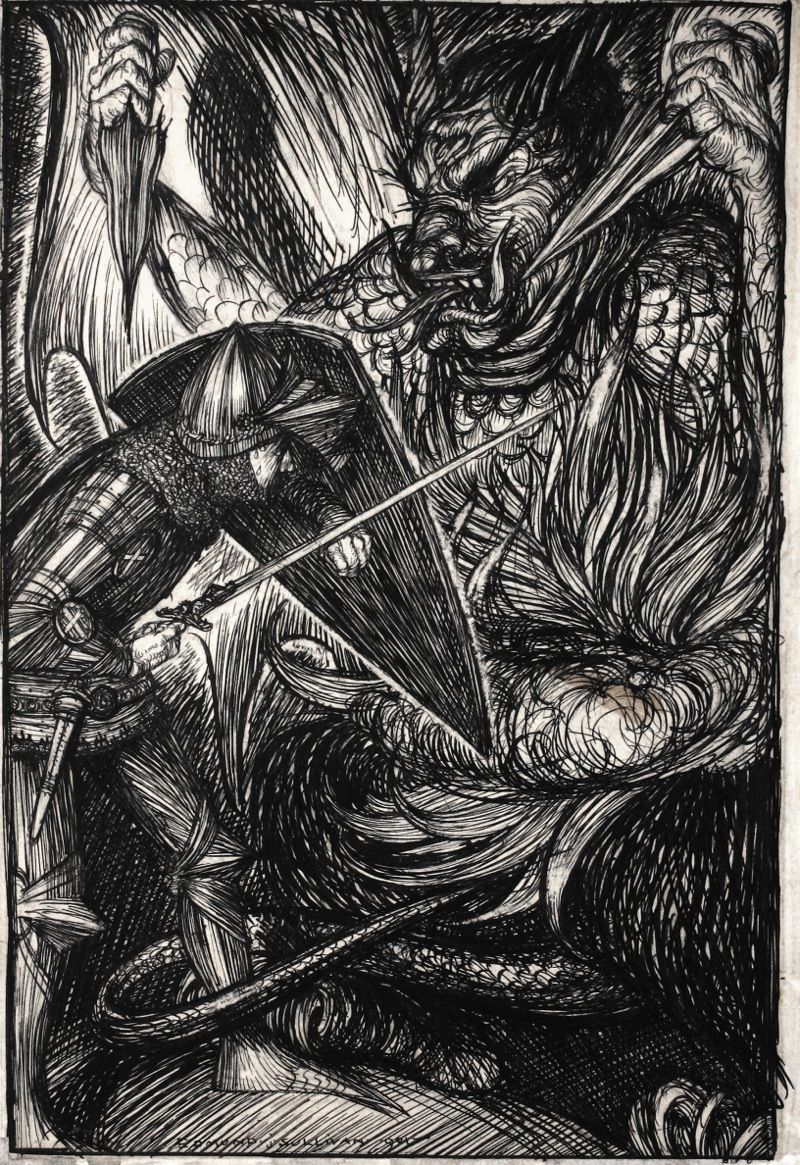
\includegraphics[width=\textwidth]{images/placeholder_image.jpg}}
\vspace*{\fill}
\clearpage

\chapter{Hibernal}

\renewcommand{\poemone}{
    \begin{figure*}[p!]
\bigskip
\ding{72}
\bigskip
\settowidth{\versewidth}{I'm not used to sleeping with someone else.}
\begin{verse}[\versewidth]
I'm not used to sleeping with someone else.\poeticmarginnote{Christmas Eve Morning}\\*
\vin I lie \sfrac{$2$}{$3$} asleep holding you stirring --\\
A hand round your heart, the prickle of your \textit{mons}.\poeticmarginnote{DM}\\
\vin All this morning I've been thinking about\\
That tender morsel of lukewarmth,\\*
\vin While the moon \& the stars wear themselves out.\nobreak\\!

The snow is quietly silting up the glasswork\\*
\vin When you open your eyes and paw my palm.\\
The flesh of your neck is like opened fruit,\\
\vin And your arms around my waist hurt.\\
Here is your tongue, and here is your navel;\\*
\vin These are your hands \& this is your side.\\!

I remember the first real girlfriend I had,\poeticmarginnote{HR}\\*
\vin Blue eyes \& a scholar's stammer.\\
She was an atheist; she was the only girl\\
\vin I ever knew who slept more deeply than me.\\
I used to hold her, of a wintertime, and\\*
\vin Trace the sign of the cross on her brow.
\end{verse}
\end{figure*}
}
\renewcommand{\poemtwo}{
    \begin{figure*}[p!]
\bigskip
\ding{72}
\bigskip
\settowidth{\versewidth}{The tide turns in the river, day becomes dusk,}
\begin{verse}[\versewidth]
The tide turns in the river, day becomes dusk,\poeticmarginnote{\textit{In Praise of Older Women}, Julika}\\*
\vin And you, as shy as a fox (or\\
My own heart), steal in\\
\vin In your mother's red silk nightdress,\\
Fringed with fur \& a hem of white satin --\\*
\vin A quaint match for your 15 years.\\!

Fire is not quenched by the dark, but\poeticmarginnote{Auden}\\*
\vin Love, sometimes, is blunted by fear:\\
You have untied the cord from your waist,\\
\vin Unstrung your softnesses into the d\'uvet,\\
But, for all my teenage desire, I\\*
\vin Could not make myself hard for you.\\!

You pressed your face against me when we kissed,\\*
\vin After, I remember, and my head swam --\\
`Young girls should show their nightgowns\\
\vin To men worthy of the name' --\\
The branches blackened \& bare in the courtyard\\*
\vin Because they could not be otherwise.
\end{verse}
\end{figure*}
}
\renewcommand{\poemthree}{
    \bigskip
\centering \ding{58}
\bigskip
\begin{quote}
\poeticmarginnote{\textarabic{محمد}}God, I am your possession, the son of your workman, the son of your washerwoman, and you hold my head in your hands. All your wishes for me are just, and your wishes are always carried out. I ask you, by every name with which you have named yourself, or which you have taught to any of your creatures, or which you have revealed in your book, or which you have kept within yourself in your knowledge of the unseen: make your book into the knocking of my heart and the brightness of my eyes, and a departure for my sorrow and a release from all distress. Amen.
\end{quote}
}
\initprintpoems

Lorem ipsum dolor sit amet, consectetur adipiscing elit. Aenean tempus ex eu dapibus cursus. Aenean orci felis, iaculis a luctus vitae, tincidunt id massa. Praesent sollicitudin quam vel quam cursus, sed sagittis elit finibus. Mauris eu tempus ante. Curabitur suscipit risus gravida, molestie arcu sit amet, cursus nunc. Donec sapien dolor, sagittis ac est quis, suscipit eleifend lectus. Sed consequat fringilla commodo.

Vivamus eget ante quis tellus ultricies aliquet. Phasellus mattis suscipit lorem eget pellentesque. Donec eget risus euismod, pulvinar felis ut, convallis quam. Cras erat velit, dapibus ac urna at, venenatis suscipit ex. Aliquam tortor metus, vestibulum facilisis accumsan ac, finibus non risus. Suspendisse at ultrices mauris. Curabitur quis accumsan erat, at consectetur tellus.

Fusce eget leo lobortis, egestas nisl quis, finibus tellus. Pellentesque aliquet id urna et malesuada. Aenean erat tortor, laoreet ac est vitae, mollis malesuada ipsum. Maecenas luctus lorem non est egestas efficitur. Aenean in lacus eu felis sodales hendrerit a vitae lacus. Curabitur eget feugiat augue. Proin consequat augue vel felis aliquet auctor. Aenean vehicula felis tellus, ac blandit massa imperdiet ut. Aenean elementum laoreet consequat. Duis egestas velit sed rhoncus euismod. Pellentesque habitant morbi tristique senectus et netus et malesuada fames ac turpis egestas.

Vivamus blandit blandit tortor, ut laoreet justo ullamcorper sit amet. Nam lobortis, enim quis gravida sagittis, metus purus finibus justo, at fringilla sem sapien suscipit sapien. Suspendisse eget lacinia justo, id volutpat purus. Suspendisse iaculis ornare odio sed gravida. Fusce lacinia turpis sed elit lobortis, at vulputate tortor dictum. Etiam placerat mi viverra finibus malesuada. Suspendisse euismod et libero vel mollis. Fusce euismod nibh odio, sit amet suscipit arcu convallis ac. Integer luctus velit ut elit condimentum, eget iaculis nisi placerat. Proin lacus augue, consectetur ut urna nec, cursus congue arcu. Ut id lacinia lacus. Nulla a malesuada sem. Nam ac pellentesque nisl, vitae placerat ipsum.

Integer fringilla rutrum nisi, quis consectetur purus tincidunt non. Maecenas sed placerat mauris. Etiam ullamcorper quam nec erat mattis, id accumsan ipsum fringilla. Maecenas tincidunt vulputate elit, eget dignissim orci porttitor ut. Cras risus dolor, consectetur nec consectetur sit amet, pellentesque sed lectus. Donec aliquam aliquam justo non porta. Vestibulum ante ipsum primis in faucibus orci luctus et ultrices posuere cubilia Curae;

Phasellus ornare ante nec est faucibus hendrerit a porttitor nulla. Nullam eget felis sit amet massa congue tincidunt eget vel lectus. Duis consequat elit a sagittis egestas. Phasellus ut interdum tortor. Suspendisse elit mi, hendrerit nec dictum non, commodo in turpis. Vestibulum tristique porta est eget fermentum. Pellentesque libero risus, dictum sed lorem ut, sollicitudin tincidunt metus. Quisque eget justo commodo, lacinia nisl nec, ornare turpis.

Phasellus dapibus nibh a mauris ullamcorper, non blandit purus maximus. Nunc dignissim felis nec est accumsan volutpat. Donec viverra efficitur tortor, a lobortis felis ultricies non. Curabitur quis fermentum urna. Vivamus finibus condimentum magna. Curabitur at leo sit amet nibh sodales molestie. Etiam sed felis eget augue gravida pretium. Etiam libero nisl, porta ut porttitor eget, luctus ac mauris.

Proin sagittis, nisi quis convallis pulvinar, mi nisi suscipit enim, id dictum ligula purus sed dui. Pellentesque sed libero ut ipsum dictum ultricies eget ut diam. Morbi eget turpis ut arcu fermentum condimentum. Praesent feugiat elit consectetur, porta nisl et, lobortis orci. Morbi interdum libero a sapien consectetur, vitae molestie magna vulputate. Etiam quis tincidunt dui. Nulla faucibus commodo posuere. Pellentesque habitant morbi tristique senectus et netus et malesuada fames ac turpis egestas. Quisque augue nulla, volutpat quis pharetra tempus, luctus fermentum purus. Sed et sem ut purus iaculis eleifend et a lectus. In sapien ante, finibus id nibh semper, tempus tincidunt mi. Quisque dapibus eget neque at bibendum. Vestibulum quis erat libero. Sed euismod tortor non nisl tincidunt mattis.

Quisque aliquet orci nisi, eget consectetur nibh ornare ut. Phasellus congue ullamcorper sapien eu elementum. Vestibulum sed maximus eros. Maecenas tincidunt pellentesque lorem eget sollicitudin. Integer et tincidunt odio. Curabitur libero sem, accumsan ac fermentum vel, tincidunt in nisl. Suspendisse in sapien quis magna tempor euismod vitae in lacus. Quisque eget magna vulputate, molestie libero at, commodo urna. Etiam feugiat velit lacinia ipsum tempor cursus. Etiam et purus eu magna volutpat hendrerit eget eget massa.

Donec at tellus velit. Proin efficitur purus non tellus porta vestibulum. Fusce purus erat, accumsan sed aliquet id, interdum et arcu. Phasellus velit libero, molestie a volutpat sit amet, mollis sit amet massa. Donec nisl mi, molestie non iaculis vitae, rutrum eget odio. Vestibulum ac pellentesque arcu, ut suscipit arcu. Phasellus et turpis pulvinar est placerat maximus sit amet eu nunc. Ut varius euismod lacinia. Fusce turpis nisi, porta ultrices condimentum eu, interdum in orci. Mauris mattis dignissim porta. Interdum et malesuada fames ac ante ipsum primis in faucibus. Duis eu suscipit odio, et vehicula leo. Nunc sollicitudin tristique facilisis. Pellentesque aliquam consequat mauris, in mattis nunc. Pellentesque et odio purus.

Phasellus vel quam nisl. Nulla metus mauris, volutpat et imperdiet ac, rutrum vitae enim. Donec ligula leo, posuere dapibus justo non, venenatis sollicitudin purus. Quisque in faucibus elit. Vestibulum hendrerit purus et ligula porta, dapibus mollis augue dapibus. Proin eu nisi a diam ultricies congue ut molestie augue. Phasellus quis nibh sit amet est auctor bibendum ac quis orci. Vestibulum tincidunt leo a massa varius, posuere scelerisque felis tristique. Nunc tempus, dui at tristique porttitor, sapien orci faucibus felis, quis finibus dui risus venenatis diam. Etiam mollis blandit risus ac vehicula. Morbi purus purus, semper at dictum sed, tempor eget mauris. Phasellus auctor, lorem ut euismod pulvinar, libero leo placerat risus, at egestas quam justo a urna. Vestibulum rhoncus nisi sit amet ipsum cursus tempor. Curabitur rutrum fringilla lobortis.

Aenean vehicula dapibus magna, quis ultrices erat ultricies vel. Vivamus fringilla nunc lectus, a pharetra odio ullamcorper vel. Aenean ac viverra ligula. Etiam et justo feugiat, feugiat eros et, mattis nisi. Mauris at rhoncus mi. Cras eu nisi nunc. Quisque id mollis arcu. Curabitur eleifend mi vitae tortor egestas porttitor. Aenean nec scelerisque quam. Sed vestibulum, sem et condimentum auctor, nisl leo porta risus, ac efficitur ex libero nec purus. Ut augue.

\clearpage

\thispagestyle{empty}
\topskip0pt
\vspace*{\fill}
{\centering
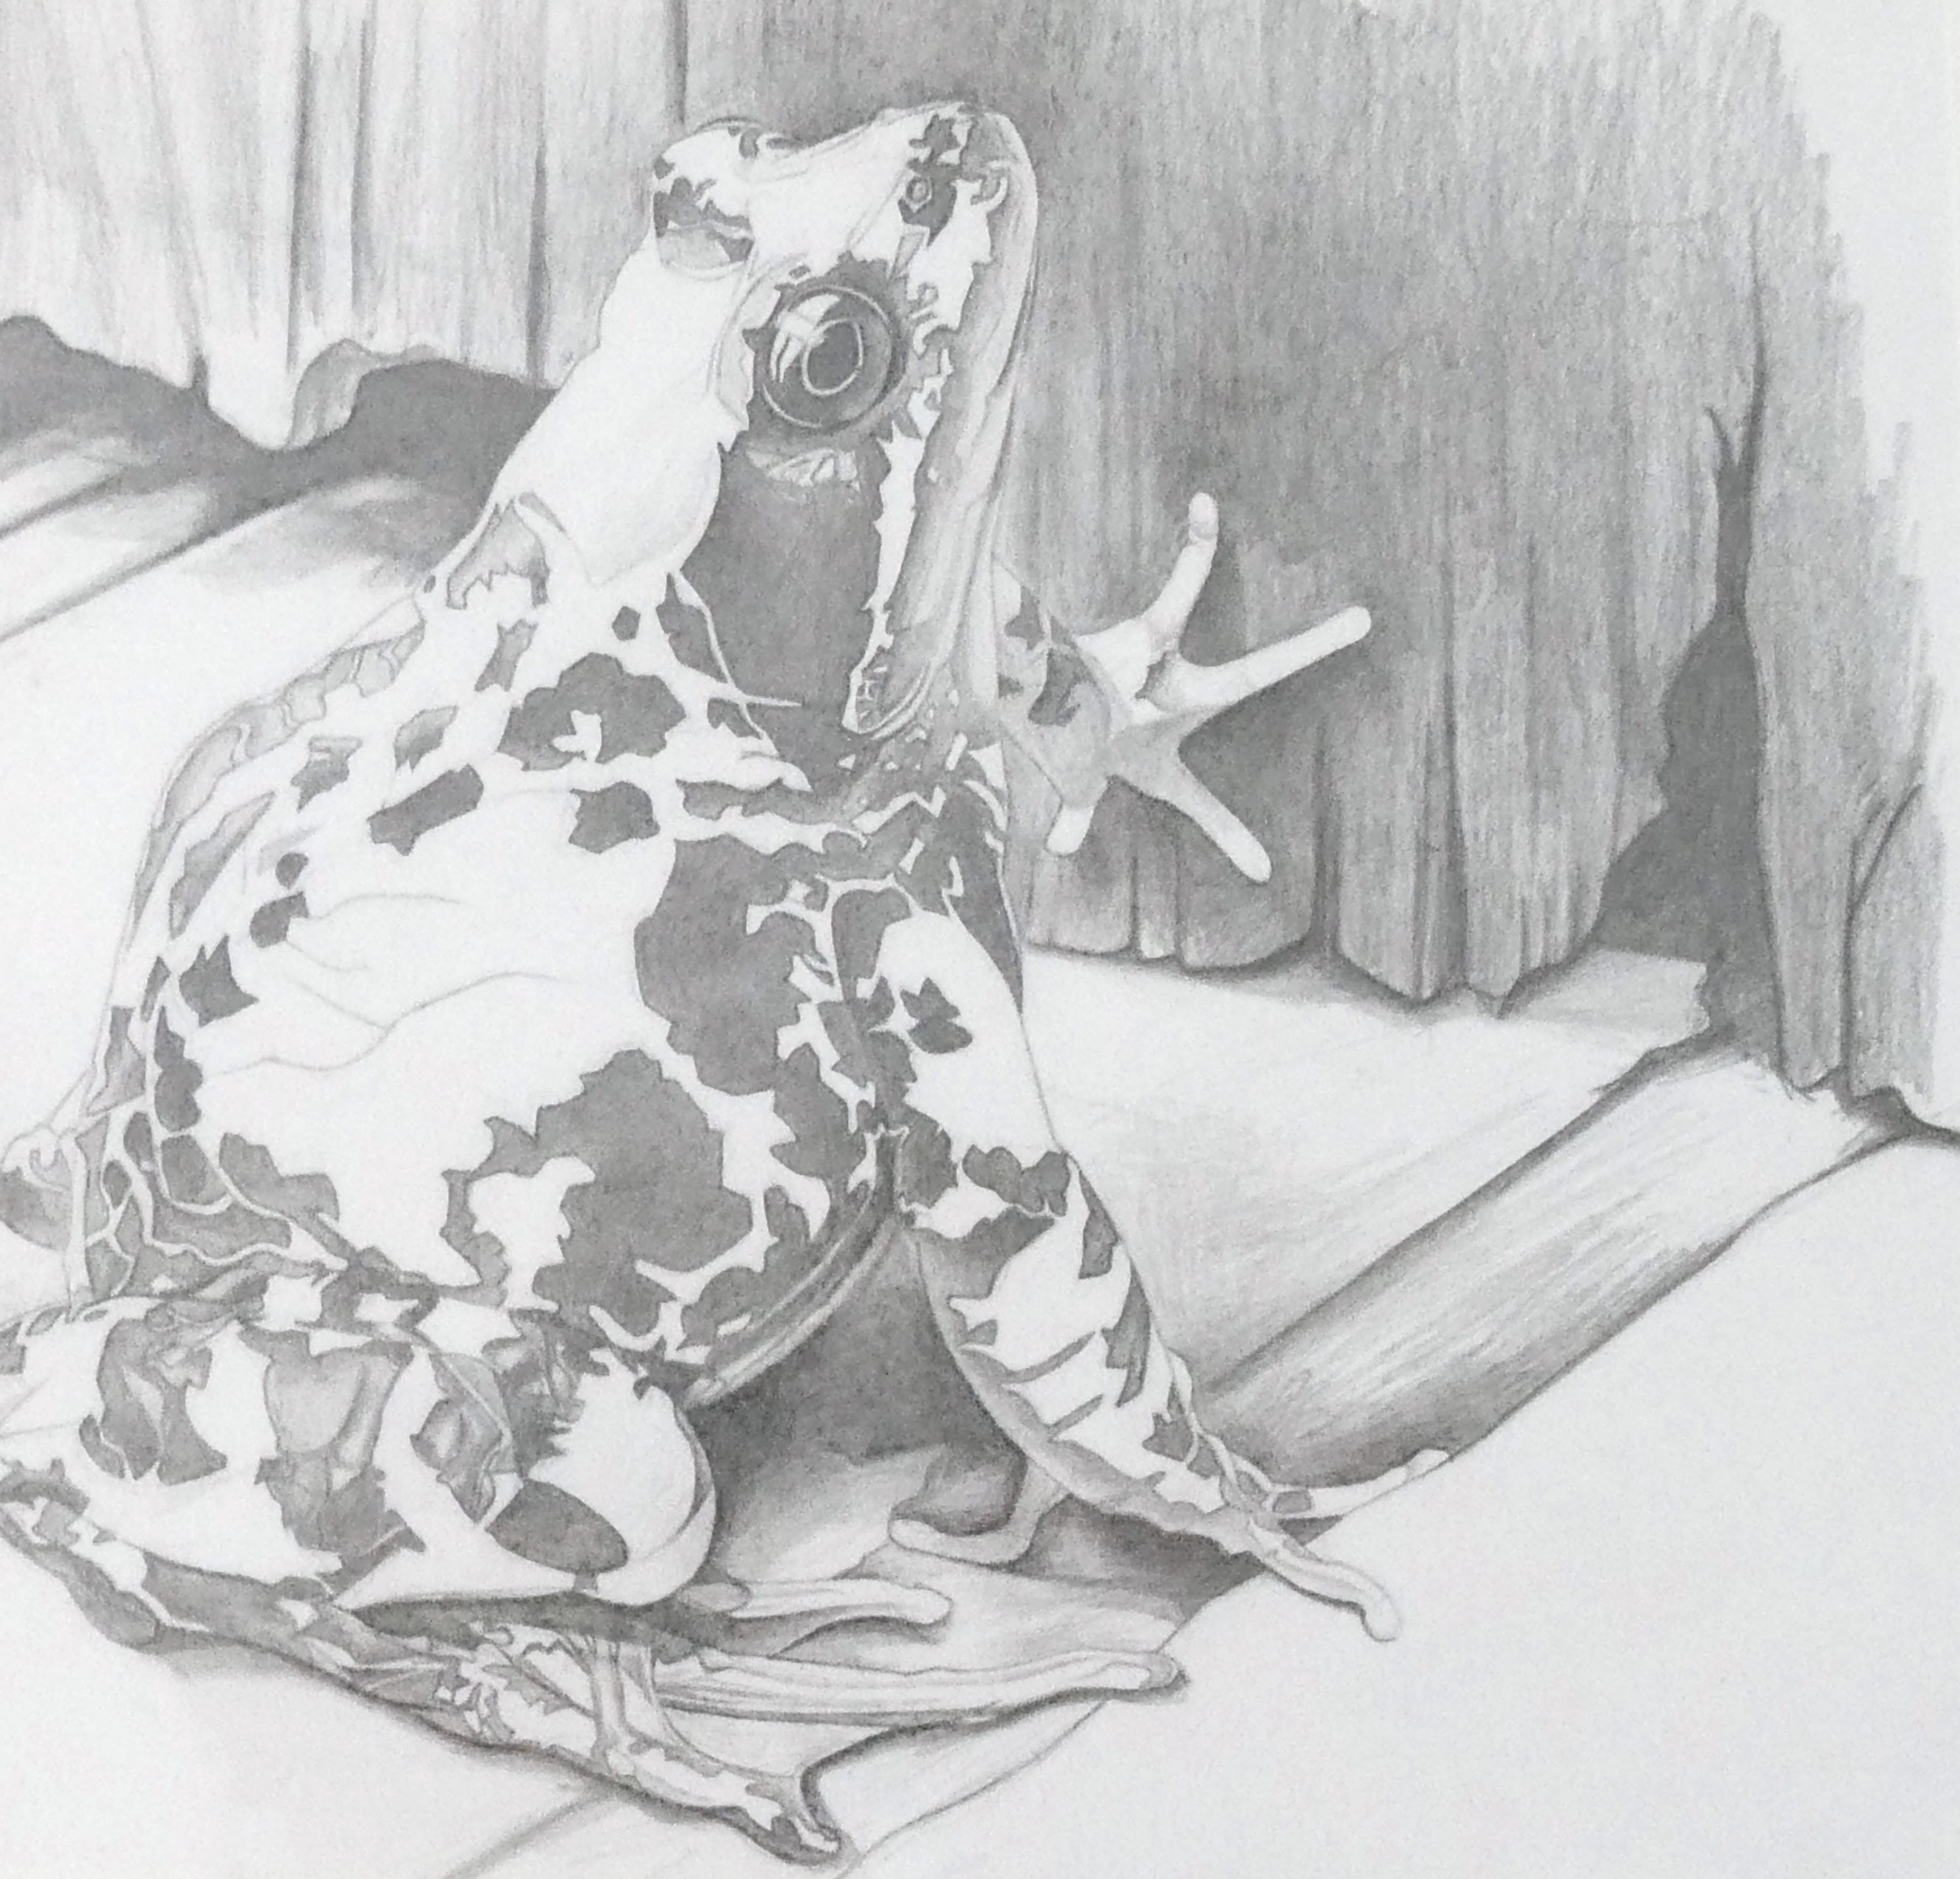
\includegraphics[width=\textwidth]{images/vernal.jpg}}
\vspace*{\fill}
\clearpage

\chapter{Vernal}

\renewcommand{\poemone}{
    \begin{figure*}[p!]
\bigskip
\ding{72}
\bigskip
\settowidth{\versewidth}{Where the sunlight catches those wine-dark stones.}
\begin{verse}[\versewidth]
I got this knife off an arab trader\poeticmarginnote{Kavadias \guillemotleft{Ένα Μαχαίρι}\guillemotright}\\*
In odds \& ends in a stall in \textsc{Algiers}.\\
I remember his hoarse voice and hollow stare,\\*
The grime staining his lips \& fingers.\\!

See that mark there. That's hand-worked sheffield steel.\nobreak\\*
Those are real rubies set into the hilt.\\
But every man who ever held its weight\\*
Ended up killing someone that he loved.\\!

A father who walked in on his young wife\\*
With his own son gutted him in the street.\\
A greek sailor sawed through his boatswain's windpipe\\*
Over a bad hand \& a packet of smokes.\\!

I keep this knife tucked into my work-belt,\\*
Where the sunlight catches those wine-dark stones.\\
And I, that care for no one in this world,\\*
Am terrified I'll only turn it on myself.
\end{verse}
\end{figure*}
}
\renewcommand{\poemtwo}{
    \begin{figure*}[p!]
\bigskip
\ding{72}
\bigskip
\settowidth{\versewidth}{Where as a younger man I'd man spent one summer.}
\begin{verse}[\versewidth]
\textsc{Bridgetown}, a night in a gale with a girl,\poeticmarginnote{Ginsberg ``Dream Record''\\~\\ES}\\*
The doctor I met on board, talking over\\
Old lost lovers and {\hoskeroe The Last Picture Show}\\
With cold beef \& chocolates \& a rough scotch.\\
Darkness. I lay in her bunk\\
And travelled in dreams back to a garden in \textsc{Rome}\\
Where as a younger man I'd man spent one summer.\\
You \& \textit{Alex} were behind the bar. It was freezing,\poeticmarginnote{RR}\\*
And the snow fell through the rich blackness into our drinks.\\!

Ah there you were, \textit{Isla}, with those curious clear blue eyes\\*
And tangled soft brown hair like a river of living bronze.\\
The time between us is nothing at all,\\*
Nor death and the river of forgetfulness.
\end{verse}
\end{figure*}
}
\renewcommand{\poemthree}{
    \bigskip
\centering \ding{58}
\bigskip
\begin{quote}
A cup of wine was offered me,\marginnote{
\includegraphics[width=12mm]{images/solomon}} and I drank it in the sweetness of my delight in you. My feet have found their furrow, my mouth its bridle. The lover has found his beloved, and Jack has his Jill. A cup of wine was offered me, because your vines were heavy with the riches therein; because whoever dips his lip into this cup tastes life itself, and whoever drinks his fill becomes immortal; and if the whole world perished, I would not. I will live by the wine of this cup forever. Alleluia.
\end{quote}
}
\initprintpoems

\noindent \textsc{I remember}, when I was seventeen, kissing a girl in a hotel restaurant in Sorrento. It was in the early hours of the morning; apart from us and another teenage couple, the place was deserted. I remember that she was wearing her pyjamas and an elegant gold pendant and a heavy, sweet perfume. She was Italian but she was a tourist like me, a Venetian; the south is really another country. The only illumination came from the lights in the street outside. Even when one puts to one side the lack of choosiness of drunk seventeen year old males, she was superlatively beautiful. She pressed her face against me and kissed me, and I put my left hand on the bare skin of her hip. She continued to kiss me, and I moved that hand further under her pyjamas. I remember the nipple of her right breast grazed the ring finger of my left hand, the first time I had touched that part of a woman since I took my mother's milk.

An\poeticmarginnote{Heraclitus v Wittgenstein} otherwise obscure philosopher wrote that one cannot step into the same river twice -- because it's not the same river and it's not the same man -- but I am strongly inclined towards the opposite point of view. All the molecules in my body -- lips, eyes and hands -- have been replaced several times since that evening in Italy, and yet these hands, in the only sense which has any practical significance, are the same hands that touched that much-missed Italian. The river is not the same thing as the water flowing through it.

\prosesep

Suppose I cut myself one afternoon while removing rust with a knife. The wound runs almost the entire length of the index finger of my left hand. If it's deep enough, it will leave an impressive scar, which, though it may fade, will be with me for the rest of my life. As with every other part of my body, all the molecules in the scar will be replaced over time. But the scar itself will remain, and if, years later, I were to point to it and say that this is where I cut myself, I would be telling the truth.

\prosesep

I have this recurring dream about my grandmother. I am standing in the living room of her old house, and she lets herself in through the front door. Where has she been? Had she not died? `Yes,' she says. `But I was only dead for a few months. That doesn't count.' (In fact, she has been dead many years, but this never occurs to me in my dream.) In life, she was not any kind of scholar, nor would she ever have become one even if she had been born into great privilege. But in my dream she utters sentences of the most dazzling sagacity, the logic of which inevitably falls apart in the morning. And the same unselfconscious kindness is there, the same quietly nurturing presence as I remember. If I try to ask her about what it feels like to be dead, she dissolves into another dream.

\prosesep

If we live again, will it be as a physical creature of some kind, or will it be as an intangible spirit? I am inclined to believe that any afterlife worthy of the name would have to take a corporeal and physical form, although without necessarily conforming to the physics of this present reality; indeed I have difficulty believing that an intangible existence is even possible in the first place. But, if my body is so indispensible to my living again, how could anyone guarantee that this new body was in fact my body, and not some kind of living wetsuit that my consciousness had stretched over itself? Does this problem actually point towards the impossibility of an afterlife?

\prosesep

When I try to imagine an eternity worth inhabiting, my mind turns inexorably towards the resurrection appearances described in the gospels. I can think of three reasons for this. (1) My upbringing was such that I instinctively think about death and the hereafter within the thought-world of Christianity. (2) The gospels seem to answer some of the philosophical objections to an afterlife -- continuity, identity, boredom, etc -- in a robust fashion. (3) The accounts of Jesus' resurrection have a compelling strangeness, not unlike an etching of an impossible object, which draw in the mind's eye long after being heard.

Assume for a moment that Jesus really did rise from the dead. Did he, on Sunday morning, inhabit the same body that the soldiers had nailed to the cross on Friday lunchtime, or was he a ghost of some sort? The gospels stress the physicality of the risen Christ. In Matthew, the women cling to his feet. In John, he famously invites one of his disciples -- who probably earned his nickname Thomas, a Greek speaker's mangling of the Aramaic word for twin, due to a striking physical resemblance to Jesus -- to put his fingers in the five wounds of the crucifixion. Luke tackles this question quite explicitly; here Jesus declares to his apostles, \textit{Touch me and see. A spirit does not have skin and bones as you see that I have.} But this body, however tangible, is not like any normal body. The risen Jesus walks through walls, appearing and disappearing at will, and barely stays in one locality for more than the length of a conversation. In the famous story of the road to Emmaus, he talks with two of his followers for what must have been several hours, but they do not recognise him -- except when, at the end of their journey, he breaks bread in a distinctive way, at which point he vanishes in plain sight. The risen Christ seems both to have re-entered his mortal body and, simultaneously, to have transmuted that same body into a new kind of matter.

\poeticmarginnote{I Cor 15.35-37}\textit{How are the dead raised? With what kind of body do they come? You foolish man. What you sow does not come to life unless it dies, and what you sow is not the body which is to be, but a bare kernel.}

One other thing: the gospels emphasise the historicity of Jesus' resurrection, Luke especially. But this only rediscovers the paradox at the heart of the resurrection from another point of view. History\poeticmarginnote{Walsh} has to do with finding similarities and differences in order to understand what happened, but, if the descriptions of the resurrection are literally true, there is nothing with which to make a comparison.

\prosesep

I\poeticmarginnote{Berryman} have no idea whether we live again. It hardly seems likely from either the scientific or philosophical point of view. \poeticmarginnote{Matthew 19.26}But all things are possible with God, and, when I try to imagine an eternity worth inhabiting, what I see are the resurrection appearances described in the gospels.

\clearpage

\thispagestyle{empty}
\topskip0pt
\vspace*{\fill}
{\centering
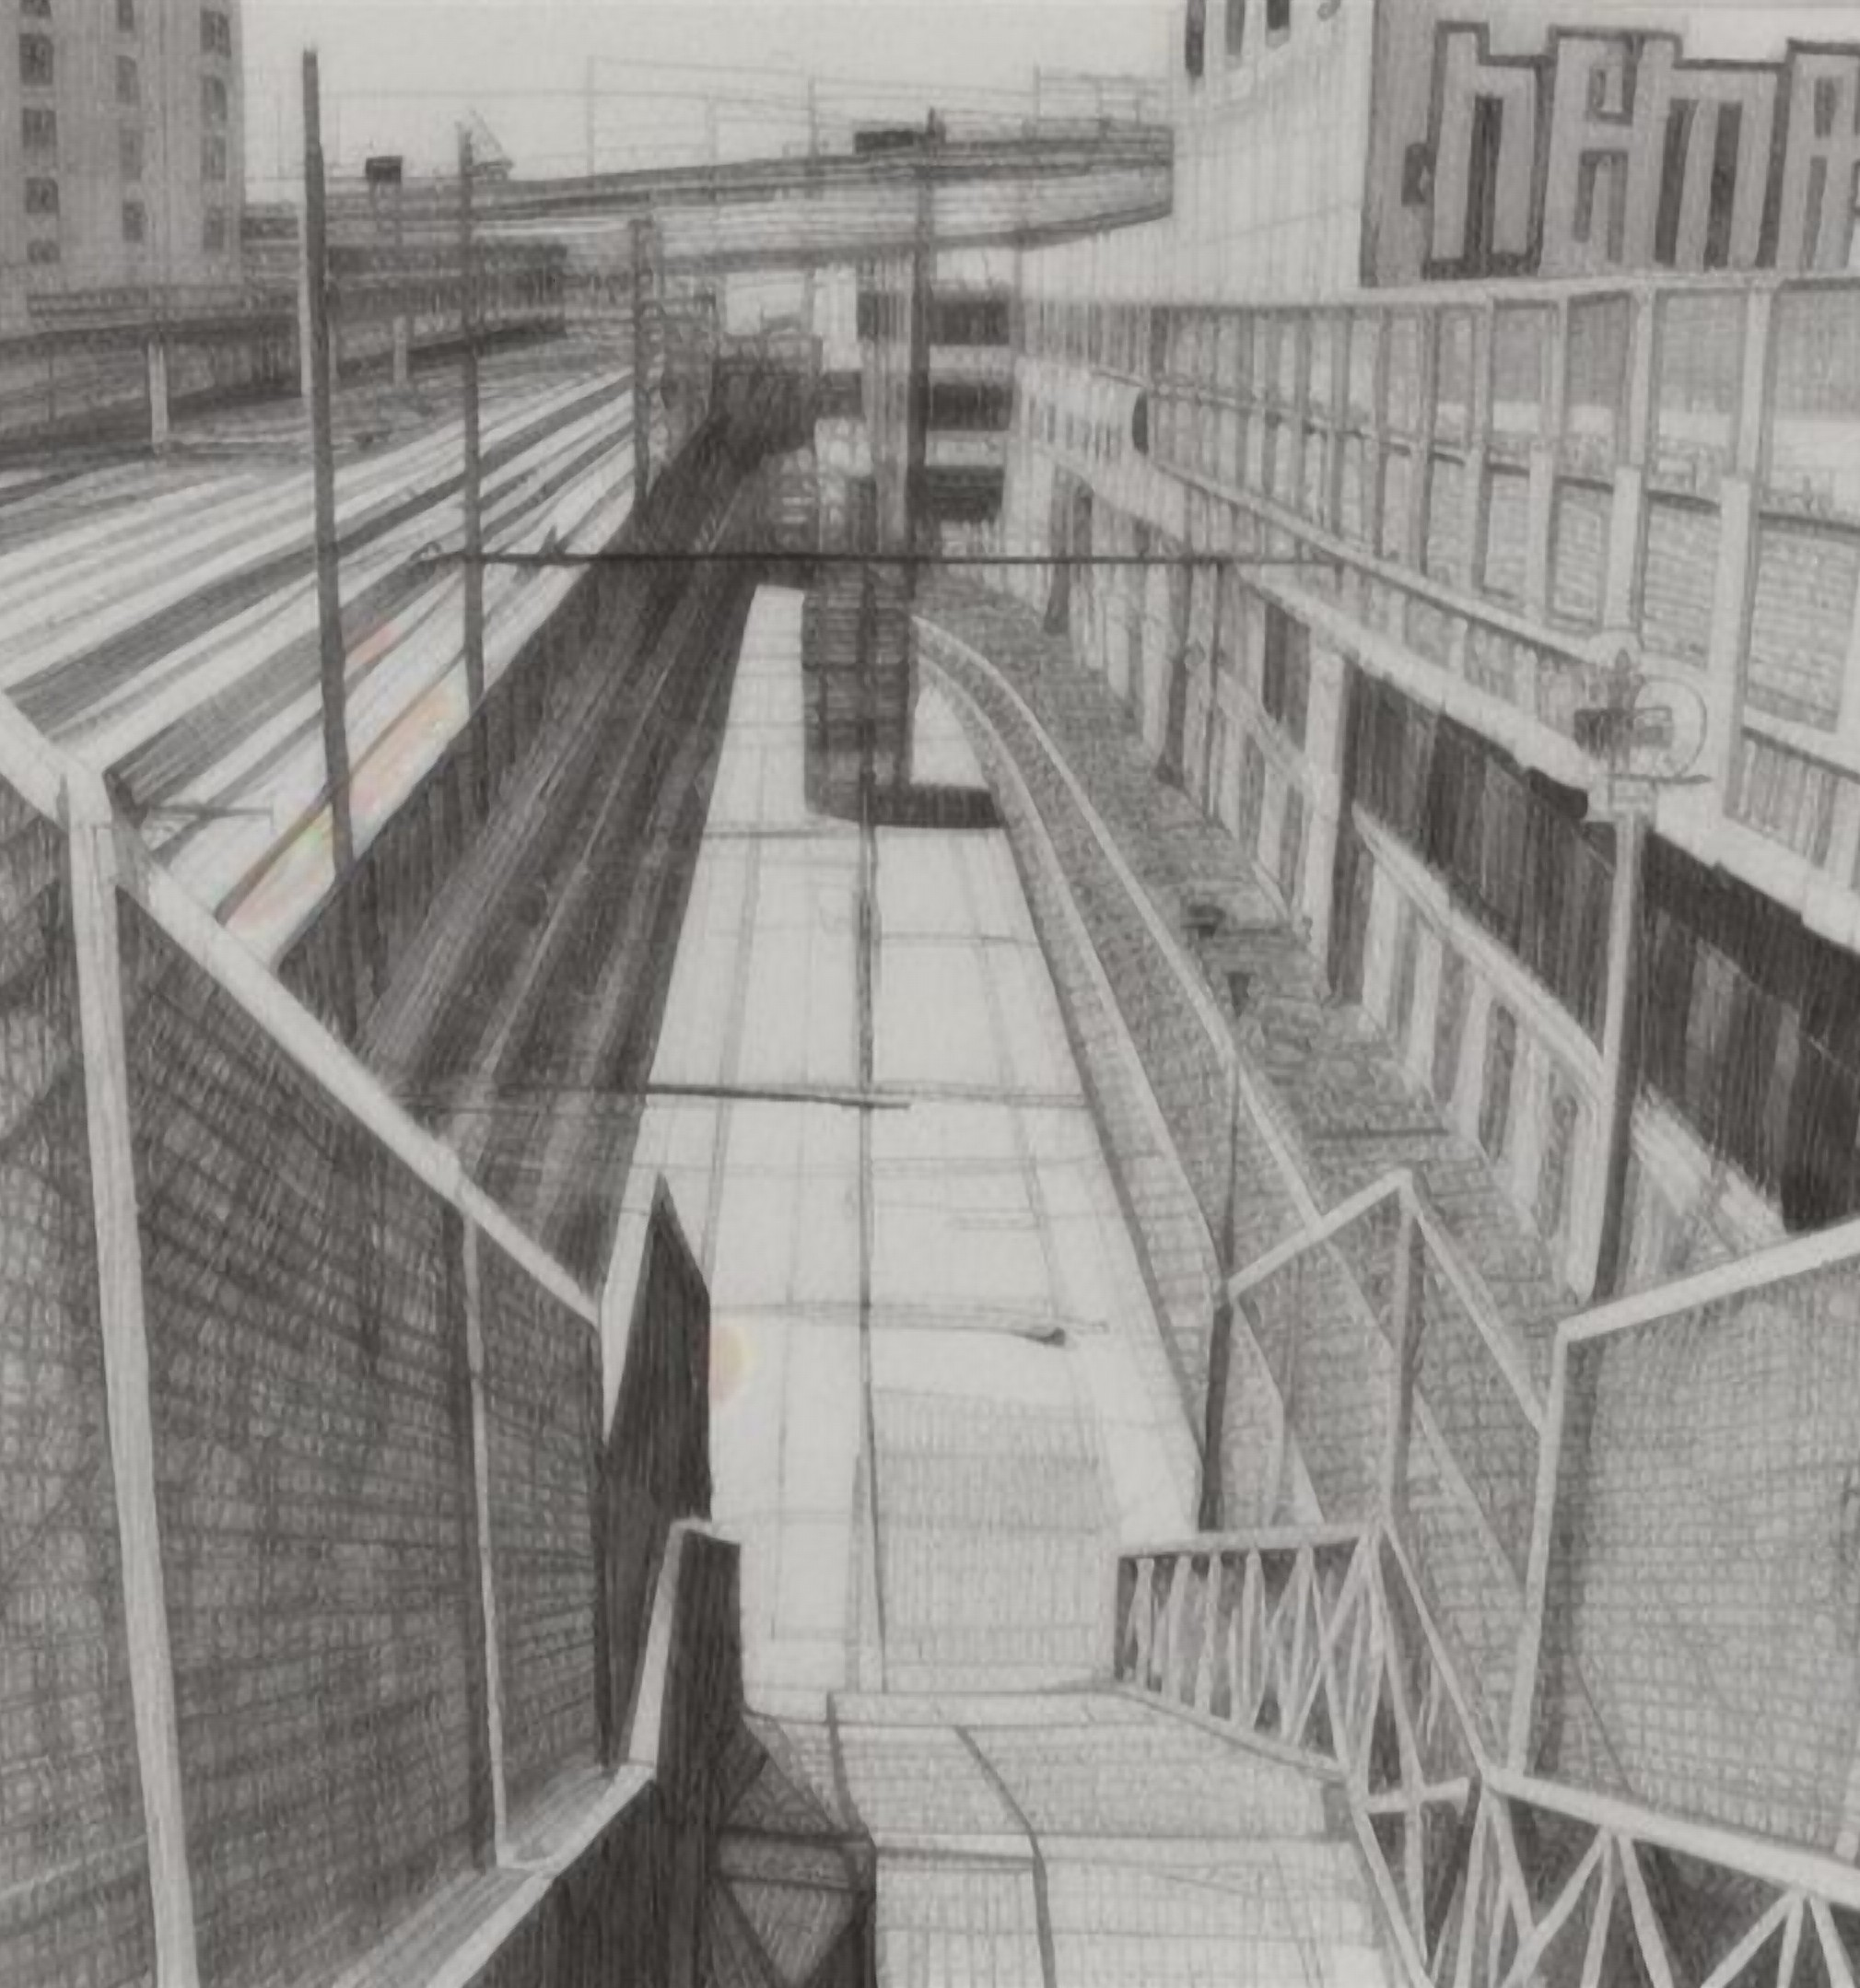
\includegraphics[width=\textwidth]{images/aestival.jpg}}
\vspace*{\fill}
\clearpage

\chapter{Aestival}

\renewcommand{\poemone}{
    \begin{figure*}[p!]
\bigskip
\ding{72}
\bigskip
\settowidth{\versewidth}{To her tapes, and sometimes smile, belle of Coach F.}
\begin{verse}[\versewidth]
She's only nine tenths beautiful,\poeticmarginnote{Blind Girl on a Train}\\*
\vin And yet we men are standing reverently around,\\
\vin \vin Watching her listening\\*
To her tapes, and sometimes smile, belle of Coach F.\\!

Her hair is tangled \& black, like black-bryony,\\*
\vin Ringletting down to her seat, beneath which\\
\vin \vin A violin case\\*
Edged with red velvet is tucked between her calves.\\!

And those cheeks, as tender as meltwater\\*
\vin And as clear, that small voice purling\\
\vin \vin More rosily than mulled wine,\\*
That six hand\poeticmarginnote{hand = 4 in} waist no soul has yet handled.\\!

But the light fails, lovers meet and journeys end.\marginnote{\footnotesize Shak}\\*
\vin She alights, to be met by her first sweetheart,\\
\vin \vin Whose head she kisses\\*
As if the world, and not her, had gone blind:\\!

And nothing matters more than a girl,\footnotetext{The poet may have had a passage from Charles Williams's \textit{Witchcraft}, quoted by Prof Auden in \textit{The Dyer's Hand}, in the back of his mind when these lines came to him, namely: `One is aware that a phenomenon, being wholly itself, is laden with universal meaning. A hand lighting a cigarette is the explanation of everything; a foot stepping from the train is the rock of all existence... Two light dancing steps by a girl appear to be what all the Schoolmen were trying to express... but two quiet steps by an old man seem like the very speech of hell. Or the other way round.'}\\*
\vin Of a velvety, late august early evening,\\
\vin \vin With her fingers\\*
In the lapels of her lover's jacket.
\end{verse}
\end{figure*}
}
\renewcommand{\poemtwo}{
    \begin{figure*}[p!]
\bigskip
\ding{72}
\bigskip
\settowidth{\versewidth}{I remember smoking hash by the railtracks}
\begin{verse}[\versewidth]
I remember smoking hash by the railtracks\\*
\vin Dribbling down from \textsc{Ponte Casalino}\\
With that giggly albino of a dutch girl\\*
\vin Who never could stay pregnant.
\end{verse}
\end{figure*}
}
\renewcommand{\poemthree}{
    \begin{figure*}[p!]
\bigskip
\ding{72}
\bigskip
\begin{verse}[0.95\textwidth]
A ghost is something -- death does not close all --\poeticmarginnote{Propertius IV.7}\\*
\vin And a spirit seeps out, untied from its body --\\
For I have seen \textit{Silvia} peering over my bedhead\poeticmarginnote{Prof Lee}\\
\vin Though we'd buried her ashes by the side of the road\\
Only that day -- as if she'd been fished out of the fire\poeticmarginnote{Leopardi}\\*
\vin And the waters of \textsc{Lethe} had not yet worn away her lips.\\!

`How can you?' she said. `How can you sleep?\\*
\vin Aren't you forgetting those nights we shared together:\nobreak\\
The zip of my sundress, worn down from overuse,\\
\vin And the scent of rose oil mingled with cigarette smoke?\\
We often made love under the railbridge,\\
\vin Our bodies warming the bare earth.\\
Alas for all those pleasures of sweet life\\*
\vin Which time \& heartache blindly washed away.\\!

`But I'll say no more about that. Water under the bridge.\nobreak\\*
\vin You paid me your respects in what you wr\'ote.\\
If you still want to make amends: bury your notebooks next to my grave,\\
\vin Plant myrtle over us both, and carve this in stone\\
(Where \textsc{Anio}'s purling fattens thirsty orchards\\
\vin And ivory, thanks to \textit{Hercules}, never yellows):\\
\textit{Here lies gold and }Silvia\textit{, bringing}\\*
\vin \textit{Glory, Father \textsc{Anio}, to your banks.}\\!

`And pay attention to the entreaties of the departed.\\*
\vin If word gets back from the dead, it must be worth knowing.\\
Daylight keeps us in chains; night sets us free,\\
\vin And \textit{Cerberus} only watches the backs of his six eyelids.\nobreak\\
Others may hold you for now;\\
\vin You'll be ashes yourself soon enough.\\
You'll be with me, and the good earth\\*
\vin Will mill each of our bones into the other's.'\\!

Thus she spoke, and laid herself beside me,\\*
\vin But when the morning came her warmth was gone.
\end{verse}
\end{figure*}
}
\initprintpoems

\noindent \textsc{Juan was} very good with women. If you have never been -- as I was when I knew him -- a sixteen year old male, free of my parents for the first time, in the intense heat of a Roman summer, you might not appreciate how close to godhood a talent with women can make a man in the eyes of his companions. But, for a young man, being good with women is not like being good with cars or horses or differential equations; those are all a means to an end, but the enjoyment of women is the summit of human existence.

Juan enjoyed plenty of women, but it would be dishonest of me if I gave you the impression that he was ever callous or possessive towards his lovers. I never saw him look at a woman as if she was his Juliet, or as if she was just another entry in a ledger of conquests. Perhaps that was his secret.

Juan was good with women, but you have probably already guessed that he stirred up a different kind of admiration in my own heart too. Just like in Solomon's dream\poeticmarginnote{I Kings 3.5-14} -- where God poured out all his other blessings because the king had the sense to ask for the one thing that was truly valuable -- Juan's talent with women seemed to be complemented by every other conceivable advantage. He was young, and I hardly need to tell you he was handsome -- but not so handsome as to obscure his generous good nature. He had a sharp mind and came from a wealthy family; when I knew him, he was taking some sort of extended holiday from an advanced degree. He was Costa Rican, but without that inflated national pride which citizens of younger countries sometimes carry within themselves; I remember one evening when we were smoking hash on a balcony, a mutual friend peeled off a ``Product of Costa Rica'' sticker from a mango and stuck it on his teeshirt, and he laughed heartily. And he also happened to possess a straightforwardly reassuring religious faith; indeed, we used to take the sacrament together at Santa Maria Maggiore, and watch the blossoms fluttering down in memory of the miraculous August snow.

\prosesep

One evening -- I remember it was a Friday -- we went for a night out in Ostia, and it happened like this. There's a train line from Basilica San Paolo to the centre of Ostia, and we bought two litres of vodka and a large carton of orange juice from a shop near the station. We took the last train out; I think in those days it left around eleven. The journey takes half an hour, and, because we had no third vessel in which to mix the juice and the alcohol, I would take a swig from the carton and Juan from the bottle, after which he would decant a glug or so from his vessel into mine. And I was astonished by the nonchalance with which he drank, as if he was imbibing nothing more caustic than lukewarm camomile tea.

In Ostia, there was a nightclub on the beach, but we rejoined Juan's friends about a hundred yards further down the shoreline, where they had built a small fire. There was a short, muscular Brazilian man, who wanted to be a boxer. There was a young Mexican, whose father had recently bought him a tiny bar in Rome proper (called La Radio) and his Italian girlfriend, who, over the course of the evening, made a number of rather funny comparisons between her boyfriend and Speedy Gonzales, which he took with very good grace. And there were also three or four young Italian men, whose names and faces I have forgotten.

Juan was friendly with the bouncers at the nightclub, so that we could come and go between the club and the campfire as we pleased. By one o'clock, Juan and myself were bored of vodka orange, and so headed for the bar for a proper drink. It was busy, and there were only a couple of bartenders; we were clearly in for a wait. But that was no matter; it gave us a chance to mingle with the girls. I got talking to a young Italian lady; her name was Vittoria. She was older than me, but only by a few months. And she was lovely to look at. She had the features one might expect from an Italian; skin half a shade darker than my own, deep brown eyes, wavy black hair. She also had exceptionally rosy cheeks which glowed a little when she smiled, even though -- except perhaps for a touch of mascara -- she was not wearing any makeup. Juan, of course, was doing his thing; I saw him talking to a girl at the other end of the enclosure. To the best of my recollection, she looked about fifteen, with light brown hair and watery blue eyes. But she stood out because of the refinement of her clothing; she wore a pearl grey cocktail dress -- a bit short, but very elegant -- paired with diamond ear studs and a pair of black stilettos. When I finally got to the bar, I asked for a \textit{gin tonica} and a vodka lime for Vittoria. I gestured to Juan asking if he would like me to get him anything, but he gestured back that he was fine.

As we walked back down the beach, I noticed some girls darting in and out of the waves, playing in the water like otters.

`\textit{Sono...?}' I asked my companion. \hspace{0.5in} {\footnotesize Are they...?}

`\textit{Completamente,}' she replied. \hspace{0.5in} {\footnotesize Completely.}

And I cursed my shortsightedness. All I could see were pink outlines in the throbbing blackness.

Vittoria had come with her brother, but she did not mind being separated from him for a bit; neither twin was overprotective like that. So we settled back down by the campfire, and spent the next few hours drinking and talking. I tried my hardest to absorb her \textit{italianit\`a}, and she put up with my weak grasp of her language most commendably.

Juan reappeared an hour before dawn, carrying a girl on his back as if he was giving her a piggyback. As he approached the fire, he laid her down for a moment on the sand. It was one of the American girls who was living in the house with us. (Her name was Heidi.) She looked nine tenths unconscious. I began to get up.

`No,' Juan said. `She's okay. I found her in the club, slumped over one of the tables. She just had a bit too much. She'll be all right.'

We took the first train from Ostia back to Basilica San Paolo, which left at about five o'clock. Vittoria was sat next to me; I finally worked up the courage to put my arm round her shoulders; and we cuddled chastely in the pre-dawn twilight for the half hour journey back into the city. We parted ways forever outside the station, and Juan and myself looked for a bus to take Heidi's mortal remains back to our house near the Ponte Casilino.

The bus was practically empty, so we took the back row. We propped Heidi against the window, and she soon passed out with her face against the glass. Naturally, Juan and myself began to talk. What was he doing while I was talking to Vittoria by the fire? Where had he been?

`I was with a girl.'

`The one I saw you with by the bar?'

`Yes.'

`And you...?'

`Yes.'

`Where?'

`We walked a bit further down the coast. I think perhaps for half a mile? There was a hotel. It was deserted. And there were plenty of loungers.'

`That's incredible.'

`That's not even the best part.' He smiled to himself. `I think she was a virgin. She was nervous and --' he pulled down his jeans to show me his underwear; on the grey cotton, there was a trail of black splodges near the crotch -- `she bled on me a bit. Anyway, she won't forget me.'

Just as he finished speaking, the bus turned and passed under the Porta Onoriana, a trio of rose-gold coloured arches, a stone's throw from the main part of the Porta Maggiore, put up in the dying years of the Western Roman Empire. It was a cloudless day, and, because it was so early, the sun was still low enough to shine directly through the archways, pouring its marvellous burgundy light down the whole length of the Via Casilina.\poeticmarginnote{I Pet 2.9} Juan and I and glanced at each other. Perhaps there was even a chuckle or a sharp intake of breath. But no words were necessary to acknowledge the moment. We passed the rest of the journey in a comfortable silence.

Heidi perked up once we were home. Juan made cheese and prosciutto omelettes for the three of us. He was, of course, an excellent cook. Then I went to my room and slept until well into the afternoon.

\prosesep

Years later, my beloved, in my parents' house in South Yorkshire, a few minutes after I had relieved you of your own virginity, I asked you if I could get you anything, and you asked for hot chocolate. I went down to the kitchen, put the kettle on, and looked through the window at the night's sky. It was about three o'clock on Christmas Day morning. For all the distance in time, climate and latitude, I could not help but think back to that morning on the Via Casilina.


\bigskip
\bigskip
\begin{center}
    \textsc{End of the First Book}
\end{center}

\end{document}
